\subsection{Opis hipotezy}\label{opis-hipotezy}

\textbf{Numer:} 1\\\textbf{Nazwa:} Ograniczenie
widoczności\\\textbf{Treść:} Czynniki ograniczające widoczność powinny
mieć duży wpływ na wzrost liczby wypadków. W szczególności groźne są
kombinacje takich czynników, przykładowo, niezwykle groźnymi warunkami
na drodze są połączenie noc i mgła, czy noc i mgła i deszcz. Można w tę
analizę włączyć jeszcze stan oświetlenia - brak oświetlenia na drodze
może dodatkowo pogarszać warunki.

\subsection{Wyniki związane z
hipotezą}\label{wyniki-zwiazane-z-hipoteza}

\textbf{Warunki pogodowe}

Udział wypadków z różnymi kombinacjami warunków pogodowych\\S - Snow\\W
- Wind\\R - Rain\\F - Fog

\begin{longtable}[c]{@{}lllllll@{}}
\toprule\addlinespace
CONDS & USA & USA \% & GB & GB \% & USA+GB & USA+GB \%
\\\addlinespace
\midrule\endhead
NONE & 1142653 & 88,17\% & 104834 & 82,98\% & 1247487 & 87,71\%
\\\addlinespace
F & 17222 & 1,33\% & 1306 & 1,03\% & 18528 & 1,30\%
\\\addlinespace
W & 445 & 0,03\% & 2798 & 2,21\% & 3243 & 0,23\%
\\\addlinespace
WF & 2 & 0,00\% & 0 & 0,00\% & 2 & 0,00\%
\\\addlinespace
R & 108652 & 8,38\% & 14463 & 11,45\% & 123115 & 8,66\%
\\\addlinespace
RF & 1444 & 0,11\% & 0 & 0,00\% & 1444 & 0,10\%
\\\addlinespace
RW & 65 & 0,01\% & 2177 & 1,72\% & 2242 & 0,16\%
\\\addlinespace
RWF & 0 & 0,00\% & 0 & 0,00\% & 0 & 0,00\%
\\\addlinespace
S & 19108 & 1,47\% & 565 & 0,45\% & 19673 & 1,38\%
\\\addlinespace
SF & 7 & 0,00\% & 0 & 0,00\% & 7 & 0,00\%
\\\addlinespace
SW & 2005 & 0,15\% & 191 & 0,15\% & 2196 & 0,15\%
\\\addlinespace
SWF & 6 & 0,00\% & 0 & 0,00\% & 6 & 0,00\%
\\\addlinespace
SR & 4283 & 0,33\% & 0 & 0,00\% & 4283 & 0,30\%
\\\addlinespace
SRF & 12 & 0,00\% & 0 & 0,00\% & 12 & 0,00\%
\\\addlinespace
SRW & 78 & 0,01\% & 0 & 0,00\% & 78 & 0,01\%
\\\addlinespace
SRWF & 0 & 0,00\% & 0 & 0,00\% & 0 & 0,00\%
\\\addlinespace
\bottomrule
\end{longtable}

\textbf{Oświetlenie}

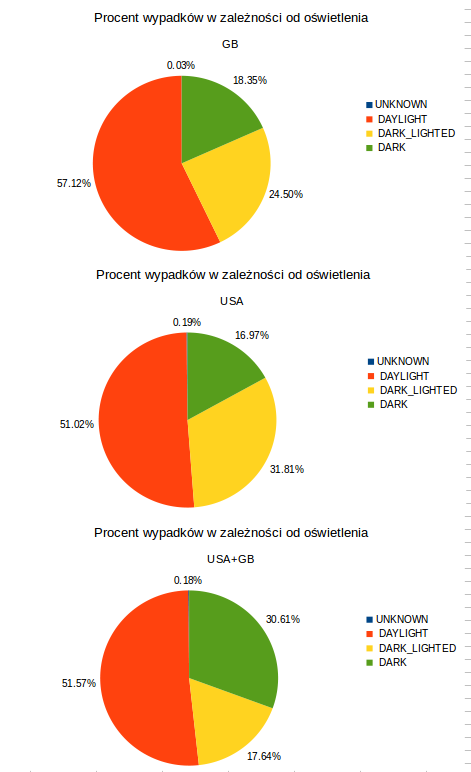
\includegraphics[width=0.8\textwidth]{images/hipotheses/lighting/lighting.png}

\subsection{Weryfikacja i wnioski}\label{weryfikacja-i-wnioski}

Analiza tabeli dotyczącej wpływu warunków pogodowych na liczbę wypadków
pokazuje, że pod tym względem hipoteza sprawdza się w ograniczonym
zakresie, prawie 80 - 90\% wypadków występuje przy pogodzie
nieutrudniającej jazdy. Warto zauważyć wyższą wartość procentową
wypadków w trakcie deszczu dla Wielkiej Brytanii - związane jest to
zapewne z faktem, że pogoda Wielkiej Brytanii jest stosunkowo często
deszczowa.

Wydaje się, że zła pogoda podwyższa nieco liczbę wypadków. W deszczowej
Wielkiej Brytanii możemy się spodziewać, że deszcz pada przez
przynajmniej 10\% czasu. Oznacza to, że udział wypadków przy pogodzie
deszczowej jest trochę wyższy niż statystycznie uzadaniony i deszcz
przyczynia się do zwiększenia liczby wypadków. Z drugiej strony analiza
\href{Hipoteza-8}{hipotezy 8} pokazuje, że rozkład wypadków w miesiącach
różni się między USA i Wielką Brytanią. W miesiącach najbardziej
deszczowych (październik, listopad, grudzień) mamy do czynienia z
podwyższeniem liczby wypadków w Wielkiej Brytanii, w USA za to
największa jest liczba wypadków w miesiącach wakacyjnych (lipiec,
sierpień), kiedy warunki do jazdy powinny być nalepsze.

Liczba wypadków przy opadach śniegu jest procentowo większy w USA. Ma to
sens, jako że w łagodnym klimacie Wielkiej Brytanii śnieg pada niezwykle
rzadko. Wartości te sugerują, że śnieg również wpływa na zwiększenie
prawdopodobieństwa wypadków. Wartości te wydają się być wyższe niż te
statystycznie uzasadnione.

Wykresy dotyczące oświetlenia pokazują, że ciemność wpływa na wzrost
liczby wypadków. Wniosek ten płynie stąd, że niewątpliwie ruch w nocy
jest mniejszy, więc prawdopodobieństwo wypadku w nocy powinno być
znacznie mniejsze. Wykresy pokazują jednak, że prawie połowa wypadków
zdarza się w ciemności, co implikuje wzrost prawdopodobieństwa wypadku w
takich warunkach. Szczególnie widoczne jest to w Stanach Zjednoczonych,
nieco mniejszy procent w Wielkiej Brytanii.

Podsumowując, trudne warunki nie wpływają aż tak bardzo na wzrostliczby
wypadków jak można by się spodziewać. Nadal znacząca większość wypadków
zdarza się w warunkach sprzyjających. Działają tu prawdopodobnie
czynniki psychologiczne - w warunkach gorszych jesteśmy ostrożniejsi i
bardziej uważamy na to co dzieje się na drodze, niwelując niekorzystny
wpływ warunków.
